\chapter{Conductance in the Kondo Regime}\label{cha:kondo_conductance}

\section{Introduction}
This chapter serves as an introduction to the Kondo effect. The background on the Kondo effect begins with a description of the first measurement that noticed a strange behaviour (resistivity minima with decreasing temperature) in impure gold wires that forty years later would become known as the 'Kondo effect'. Similar to the historical timeline of Kondo measuremets, the quantum dot is introduced as an exciting platform to explore Kondo physics due to high degree of in-situ tunability. 


\afterpage{\clearpage}
\section{Kondo Effect in Bulk Materials}


In the 1930s', it was found that in impure gold wires, the resistivity would surprisingly increase at low temperatures~\cite{de_haas}. It was expected that due to electron-phonon scattering, the resistivity would decrease with $\mathrm{T^5}$ before saturating at some non-zero resistivity Fig.~\ref{fig:ch2/kondo_bulkmetal}. Over the coming years it was found that metals with  magnetic impurities had a similar behaviour~\cite{still_irresistible}.


\begin{figure}[!hbt]
  \begin{center}
%% includegraphics: comment the following if not using the graphicx package
    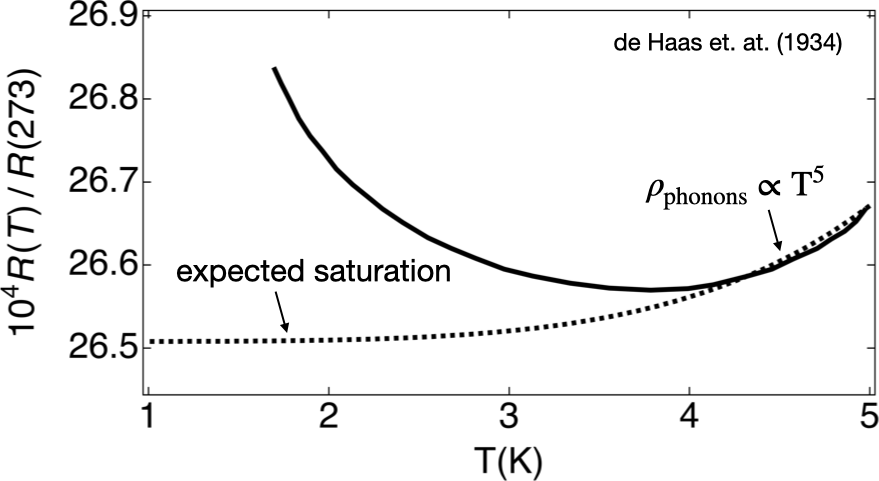
\includegraphics[width=0.9\textwidth]{figures/ch2/crop_FiguresMaster.008.png}
    \caption[Kondo effect in bulk materials]{\label{fig:ch2/kondo_bulkmetal} 
    % For some options that work with pdf\LaTeX, please see this discussion:
    %   \url{http://tex.stackexchange.com/questions/11839}.  
    Temperature dependence of the resistivity, $\rho$. Due to electron-phonon scattering, the resistivity decreases as $T^5$. Due to the Kondo effect, the resistivity will reach a minima before it starts increasing logarithmically with decreasing $\mathrm{T}$. The data used for this figure has been obtained from~\cite{de_haas}.
      }
  \end{center}
\end{figure}

\begin{figure}[!hbt]
  \begin{center}
%% includegraphics: comment the following if not using the graphicx package
    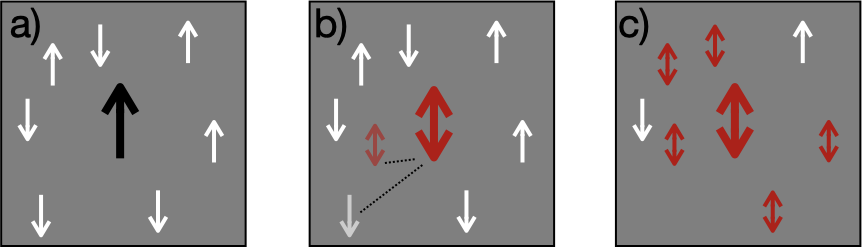
\includegraphics[width=0.9\textwidth]{figures/ch2/crop_FiguresMaster.009.png}
    \caption[Kondo effect in bulk materials]{\label{fig:ch2/kondo_bulkdiagram} 
    % For some options that work with pdf\LaTeX, please see this discussion:
    %   \url{http://tex.stackexchange.com/questions/11839}.  
    (\textbf{a}) A single magnetic impurity (black arrow) is surrounded by conduction electrons (white arrow). (\textbf{b}) Conduction electrons scatter off the localised state resulting in a possible spin flip of both particles, leaving the particles entangled. (\textbf{c}) Continued scattering events build a macroscopic coherent state known as a 'Kondo singlet' .
      }
  \end{center}
\end{figure}

It took until 1964 for a theoretical explanation of the resistivity minima~\cite{jun_kondo}. Jun Kondo showed that magnetic impurities give rise to an alternative scattering process involving a temporary exchange of spin states between the magnetic impurity and surrounding conduction electrons.  
It was shown that the Kondo system could be modelled by a magnetic impurity interacting with a bath of spins. When doing so, a second order term in the perturbation results in a large correction at low $\mathrm{T}$, leading to a logarithmic increase in resistivity with decrease in temperature. 

Fig.~\ref{fig:ch2/kondo_bulkdiagram} visualises the build up of the bond between the magnetic impurity and the free conduction electrons. 
Fig.~\ref{fig:ch2/kondo_bulkdiagram}b) shows a scattering event which may or may not result in the spin flip of the conduction electron and the magnetic impurity, leaving the two particles entangled. Continued scattering events between the magnetic impurity and conduction electrons will result in a macroscopic state as the conduction electrons are correlated with the magnetic impurity Fig.~\ref{fig:ch2/kondo_bulkdiagram}c). This is known as a 'Kondo singlet' or 'Kondo cloud'. It is found that a single parameter sets the scale for the existence of the Kondo singlet, the Kondo temperature $\mathrm{T_k}$. 

 








% \afterpage{\clearpage}
\section{Kondo Effect in Quantum Dots}

\begin{figure}[!hbt]
  \begin{center}
%% includegraphics: comment the following if not using the graphicx package
    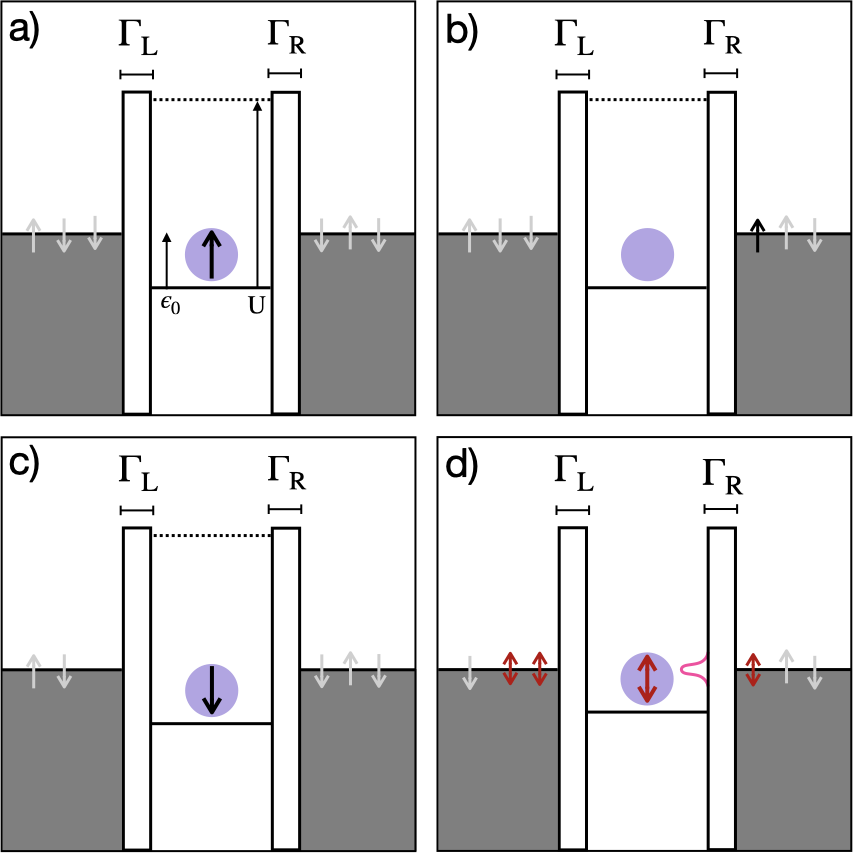
\includegraphics[width=0.75\textwidth]{figures/ch2/crop_FiguresMaster.010.png}
    \caption[Kondo effect in a quantum dot: Coulomb blockade energy diagrams]{\label{fig:ch2/kondo_dot_diagram} 
    % For some options that work with pdf\LaTeX, please see this discussion:
    %   \url{http://tex.stackexchange.com/questions/11839}.  
    A Coulomb blockade energy diagram picture of a Kondo singlet formation in a quantum dot. Here the dot acts as the localised spin. The dark grey represents the continuous energy level of electrons in the leads. The white rectangles represent tunnel barriers between the quantum dot and leads. The rate of tunneling is described by the parameter $\Gamma$, the wider (narrower) the barrier, the smaller (larger) the rate of tunneling. (\textbf{a}) The quantum dot has a one spin-degenerate energy level $\mathrm{\epsilon_0}$ occupied by a single electron. The next energy level is separated by the charging energy, $\mathrm{U}$. From Figure~\ref{fig:ch1/dot_intro} we expect zero conductance through the quantum dot. (\textbf{b},\textbf{c}) depict a possible virtual tunneling event, where the spin-up electron tunnels out of the dot and a spin-down electron tunnels into the dot within a short time. (\textbf{d}) These virtual tunnel events involving spin-flips lead to a correlated state, the Kondo-singlet. This state can be pictured as a narrow density of states formed at the Fermi energy of the leads. If a Kondo singlet has been formed, we will measure enhanced conductance though the quantum dot even as the energy level of the dot is below the energy level of the leads. Note: The formation of the Kondo singlet requires an odd number of electrons in the quantum dot.
      }
  \end{center}
\end{figure}

Until the late 1990s, the Kondo effect had been mainly explored by theoretical solid-state physicists due to the difficulty of experimentally controlling the Kondo state~\cite{kondo_review}. 
However, after advances in quantum dot design, the potential for precise in-situ control was irrestible and the first measurement of a Kondo singlet was in 1998~\cite{goldhaber_first_kondo}. It was around this time that scanning  tunnelling microscope (STM) was also used to study the Kondo effect~\cite{stm_kondo}.
In quantum dots, it is an odd number of electrons in a quantum dot that act as the magnetic impurity in bulk metals. Similar to bulk metals, the conduction electrons in the 2DEG can interact with the net spin in the quantum dot. The advantage of studying the Kondo effect in quantum dots comes from the in-situ control over the coupling strength, voltage bias, and energy level of the impurity.
The formation of a Kondo singlet in quantum dots can be visualised similarly to that in bulk metals Fig.~\ref{fig:ch2/kondo_dot_diagram}. 
If the dot energy of the quantum dot is below the Fermi energy, we do not expect the electron to tunnel out of the dot as there are no available empty energy levels. However, it so happens that the electron in the dot can tunnel into the leads Fig.~\ref{fig:ch2/kondo_dot_diagram}\textbf{b}) as long as another electron tunnels into the quantum dot within the timescale limited by Heisenberg’s uncertainty principle Fig.~\ref{fig:ch2/kondo_dot_diagram}\textbf{c}). This can result in a spin flip of the impurity. Many of these virtual tunneling events will lead to the formation of a singlet state, increasing the density of states at the Fermi level Fig.~\ref{fig:ch2/kondo_dot_diagram}\textbf{d}). 

 
\begin{figure}[!hbt]
  \begin{center}
%% includegraphics: comment the following if not using the graphicx package
    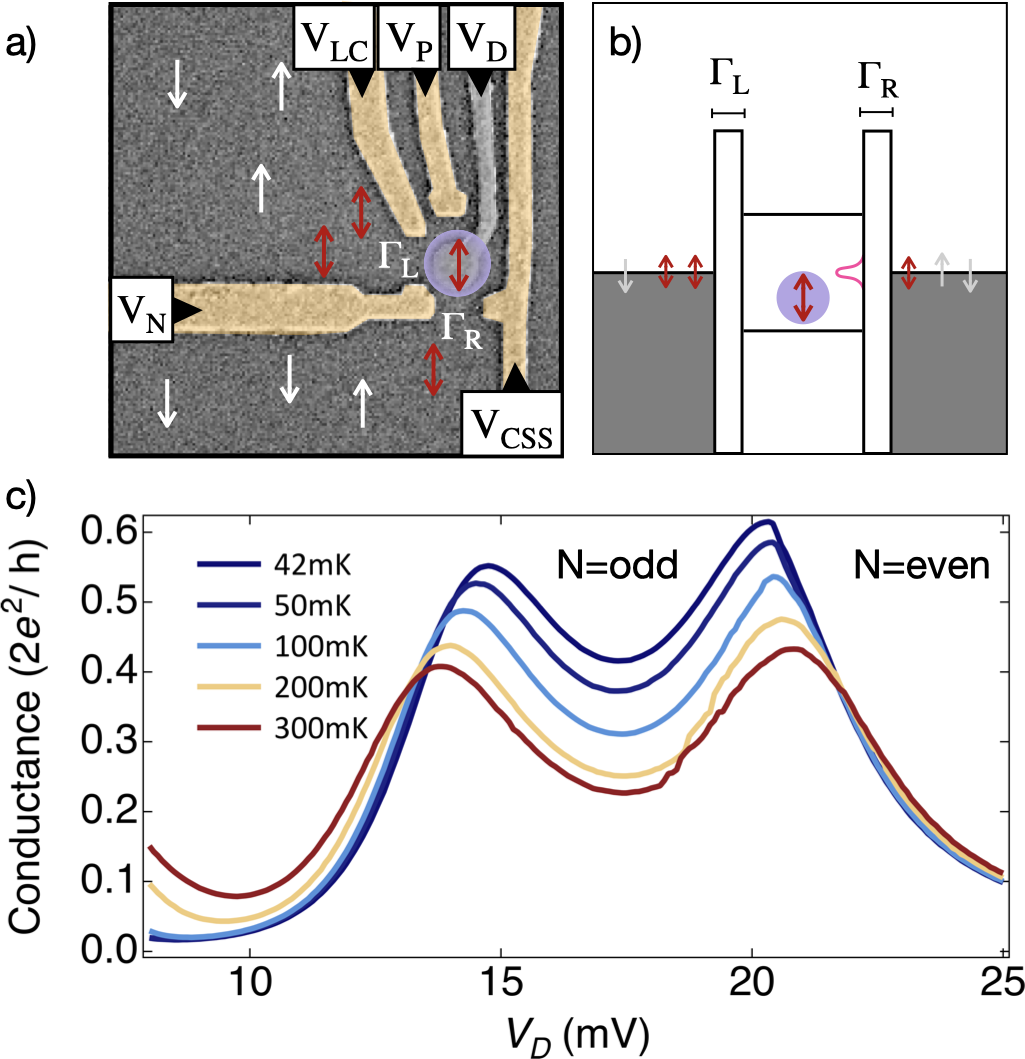
\includegraphics[width=0.9\textwidth]{figures/ch2/crop_FiguresMaster.011.png}
    \caption[Kondo effect in a quantum dot in the Kondo regime]{\label{fig:ch2/kondo_regime_conductance} 
    % For some options that work with pdf\LaTeX, please see this discussion:
    %   \url{http://tex.stackexchange.com/questions/11839}.  
    (\textbf{a}) An SEM image of the gates used to define a quantum dot. The dot contains an odd number of electrons and the tunnel barriers are tuned so that a Kondo singlet is formed. (\textbf{b}) A Coulomb blockade energy diagram picture of a Kondo singlet. As the dot energy falls below the energy level of the leads, there is enhanced conductance due to virtual tunneling events through the quantum dot. (\textbf{c}) Data showing the temperature dependence of conductance through a quantum dot when a Kondo singlet is formed. In the even occupied sides conductance decreases as the temperature is lowered. On odd occupation, a Kondo singlet forms and conductance increases with decreasing temperature.}
  \end{center}
\end{figure}


 Contrary to the resistivity increase in bulk metals, the presence of a Kondo singlet leads to enhanced conductance through the quantum dot as the dot energy fell below the energy level of the source and drain leads Fig.~\ref{fig:ch2/kondo_regime_conductance}. The enhanced conductance increases as the system temperature fall below the Kondo temperature $\mathrm{T_k}$. Similar to bulk metals, the existence of the Kondo effect in quantum dots is set by the system temperature being lower than the Kondo temperature $\mathrm{T_k}$. When the dot energy is far below the Fermi level in the leads, the Kondo temperature depends exponentially on the depth of that level~\cite{goldhaber_mv}, 

\begin{equation}\label{eq:kondo_temp}
  \mathrm{T_K} = 
  \frac{\sqrt{\Gamma \mathrm{U}}}{2}
  \exp{\pi \epsilon_0 (\epsilon_0 + \mathrm{U})/\Gamma\mathrm{U}}
\end{equation}

where $\mathrm{\Gamma = \Gamma_L + \Gamma_R}$. The Kondo temperature also depends on the strength of coupling i.e. the stronger the coupling, the larger the Kondo temperature. This expression for the Kondo temperature only holds in the 'Kondo regime'. The Kondo regime is characterised by $\tilde{\epsilon}_0<<-0.5$ where $\tilde{\epsilon}\equiv \epsilon_0/\Gamma$. Many of the early measurements on the Kondo effect in quantum dots used very strong couplings so the system temperature remained below the Kondo temperature deep into the Kondo regime~\cite{kondo_unitary}. Such studies examined temperature dependence of the conductance in the Coulomb blockade valley where the conductance dependence on temperature is non-monotonic and has a minimum at finite temperatures~\cite{Pustilnik2004}.  It was found that in the Kondo-regime, the Kondo temperature Eq.~\ref{eq:kondo_temp} sets a new many body scale. The Kondo temperature can be used to normalise the conductance such that it is independant of other energy scales $\Gamma$, $\mathrm{U}$ and $\tilde{\epsilon}_0$.

\begin{equation}\label{eq:kondo_conductance}
  \mathrm{G(T)} =
  \mathrm{G_0}
  \left(
  \frac{\mathrm{T_k'^{2}}}{\mathrm{T^2} + \mathrm{T_k'^{2}}}
  \right)^\mathrm{s}
\end{equation}

where $\mathrm{T_k'^{2}} = \mathrm{T_k}/\sqrt{2^{\mathrm{1/s}}-1}$ and $\mathrm{s} \approx 0.20$ for a spin-1/2 system in the Kondo regime~\cite{goldhaber_mv}. The parameter $\mathrm{s}$ determines the steepness of the conductance drop with increasing temperature. The one parameter scaling of the conductance in the Kondo-regime is used as one of the demonstrations of the Kondo effect. Other measurements include a zero-bias peak in the Coulomb blockade valley~\cite{kondo_unitary} and a splitting of this zero-bias peak with magnetic field [REF XXX].  

Other efforts have been made to explore the Kondo effect with weaker coupling where the conductance in the middle of the Coulomb blockade valley does not follow the surprising increase with decreasing temperature~\cite{goldhaber_mv}. This regime of weaker coupling is the focus of the next chapter. 

% Other efforts were made to explore the Kondo effect with weaker coupling in the so-called 'mixed-valence regime'. This regime is characterised by $-0.5<<\tilde{\epsilon}_0<<0$ and is the focus of the next chapter. 



